\chapter*{Capitolo 4}
\addcontentsline{toc}{chapter}{Capitolo 4}


\section*{Risultati}
\addcontentsline{toc}{section}{Risultati}


\section*{DPDK}
\addcontentsline{toc}{section}{DPDK}
I Test con DPDK hanno riportato i seguenti risultati.
I risultati di ricezione e trasmissione virtuale riguardano l'effettivo throughput generabile da DPDK, ovvero la capacità limite di generazione e ricezione di pacchetti che si ha per la specifica infrastruttura.
I risultati di ricezione reale invece indicano la quantità di dati effettivamente ricevuti dalla scheda di rete e registrati con il programma \textbf{bwm-ng} \cite{noauthor_bwmng} sul computer host. Appare chiaro che disponendo di una scheda di rete Gigabit è impossibile ricevere un flusso di dati superiore a questo valore.
Parte dei test in macchina virtuale sono stati eseguiti anche attivando il PCI Passthrough, ma i risultati riportati si discostano di pochi Mbit/s dai test con le interfacce MacVTap e quindi non sono riportati. Questo distaccamento minimo è possibile grazie alla grande efficienza dei driver MacVTap in combinazione con il Kernel Bypassing effettuato da DPDK.

\vspace{1cm}
\begin{center}
\begin{tabular}[h!]{ |c|c|c|c|c| } 
\hline
\rule{0pt}{4ex}
Infrastruttura & Trasmissione virtuali & Ricezione virtuali & Trasmissione effettivi & Ricezione effettivi \\
\hline
\rule{0pt}{4ex}
\textbf{{Figura \ref{fig:dpdk_vm1}}} & 800Mbit/s & 800Mbit/s & 800Mbit/s & 800Mbit/s \\ 
\hline
\rule{0pt}{4ex}
\textbf{{Figura \ref{fig:dpdk_vm2}}}& 3Gbit/s & 3Gbit/s & 1Gbit/s & 1Gbit/s\\ 
\hline
\rule{0pt}{4ex}
\textbf{{Figura \ref{fig:dpdk_lan2}}} & 10Gbit/s & 1Gbit/s & 1Gbit/s & 1Gbit/s\\
\hline
\end{tabular}
\end{center}
\vspace{1cm}

\label{fig:dpdk_differences}

\subsection*{Considerazioni}
\addcontentsline{toc}{subsection}{Considerazioni}
\leavevmode\newline
Nei test mostrati in \textbf{{Figura \ref{fig:dpdk_vm1}}}
 la velocità di trasmissione è ridotta rispetto ai test successivi perché DPDK è CPU intensive. In questo caso infatti sullo stesso host ci sono due istanze running di DPDK, una per l'invio e una per la ricezione dei pacchetti che, secondo la semantica dei Poll Mode Drivers, chiedono in modalità polling alla CPU la presenza di pacchetti da processare.
\leavevmode\newline
\\
In \textbf{{Figura \ref{fig:dpdk_vm2}}} invece i test presentano un risultato migliore in termini di performance a livello Data Plane: in questo caso gli interrupt generati dai Poll Mode Drivers sono su due processori diversi in due macchine virtuali diverse risultando in una gestione generalmente migliore. In questo caso, inoltre, ogni macchina virtuale ha due core dedicati, in contrapposizione al precedente caso di singola macchina virtuale con due core totali.
\leavevmode\newline
\\
Nei test in \textbf{{Figura \ref{fig:dpdk_lan2}}} siamo in condizioni reali, ovvero in una rete domestica con un router che si occupa di amministrare i pacchetti spediti dal dispositivo con DPDK. In questo caso, disponendo di una grande capacità di calcolo, ovvero con 4 core dedicati alla generazione dei pacchetti, è possibile riuscire a generare fino a 10 Gbit/s. Non è possibile far passare tale quantità di dati al secondo attraverso il router a causa del limite fisico della scheda di rete. L'invio dei pacchetti infatti sarà limitato alla capacità massima di invio di 1Gbit/s tipico delle NIC standard. Anche se la scheda di rete fosse capace di generare un tale bitrate, il router genererebbe ``bottleneck", disponendo anch'esso di porte Gigabit Ethernet.
La ricezione virtuale e fisica in questo caso, quindi, coincideranno.

\subsection*{Problematiche}
\addcontentsline{toc}{subsection}{Problematiche}
Durante il testing di DPDK, uno dei problemi maggiori è stato monitorare l'invio dei pacchetti senza il tool Pktgen. Sfruttando il Kernel Bypass, DPDK si stacca completamente dal Kernel e si astrae nello user-space, quindi è praticamente impossibile riuscire a leggere i pacchetti in ricezione e in trasmissione se non con dei programmi che sfruttano le librerie apposite di DPDK in user-space. Nei test in macchina virtuale è stato però comunque possibile riuscire a leggere il traffico che DPDK generava, leggendo il buffer delle interfacce MacVTap, potendo monitorare l'effettivo throughput anche da una fonte esterna a Pktgen.


\section*{P4}
\addcontentsline{toc}{section}{P4}

I test con P4 hanno riportato i seguenti risultati.
In questo tipo di setup i test sono stati eseguiti solo in una rete interna tra macchine virtuali, quindi non è presente la distinzione tra throughput effettivo e virtuale. Ogni switch riceve i pacchetti, li accetta e li inoltra se l'header fa match con l'header ethernet o l'header IPv4.

\vspace{1cm}
\begin{center}
\begin{tabular}[h!]{ |c|c|c| } 
\hline
\rule{0pt}{4ex}
Infrastruttura & Trasmissione & Ricezione \\
\hline
\rule{0pt}{4ex}
\textbf{{Figura \ref{fig:p4_basic}}} & 830Mbit/s & 830Mbit/s \\ 
\hline
\rule{0pt}{4ex}
\textbf{{Figura \ref{fig:p4_double}}} & 425Mbit/s & 425Mbit/s \\ 
\hline
\end{tabular}
\end{center}
\vspace{1cm}

\FloatBarrier
\begin{figure}%
    \centering
    \subfloat[\centering H1]{{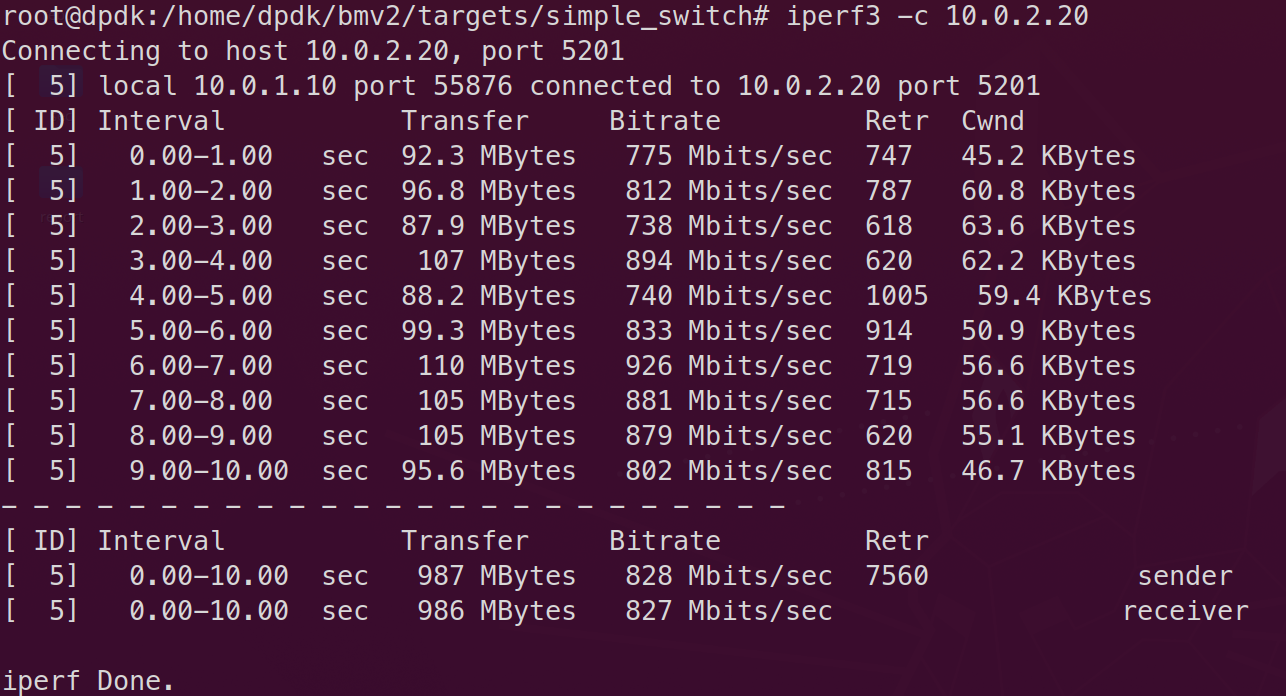
\includegraphics[width=7.5cm]{images/h1_p4basic_patrick.png} }}%
    \qquad
    \subfloat[\centering H2]{{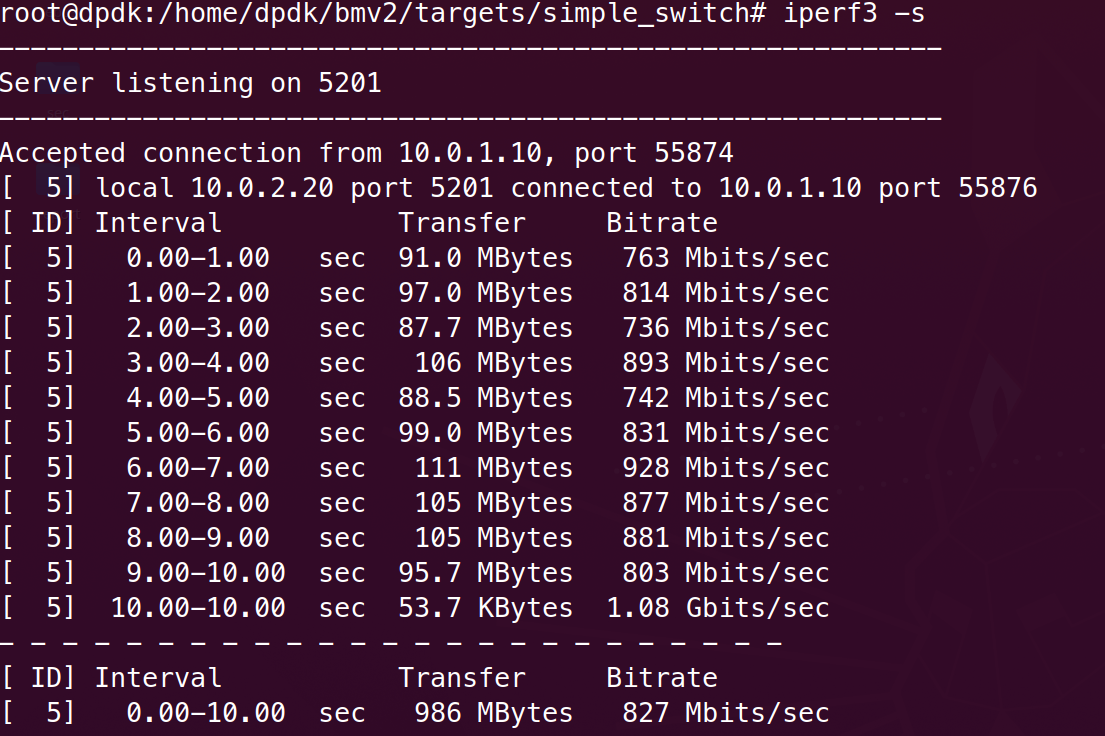
\includegraphics[width=7cm]{images/h2_p4basic_patrick.png} }}%
    \caption{P4 single switch}%
    \label{fig:h1_p4basic_patrick}%
\end{figure}
\FloatBarrier


\FloatBarrier
\begin{figure}%
    \centering
    \subfloat[\centering H1]{{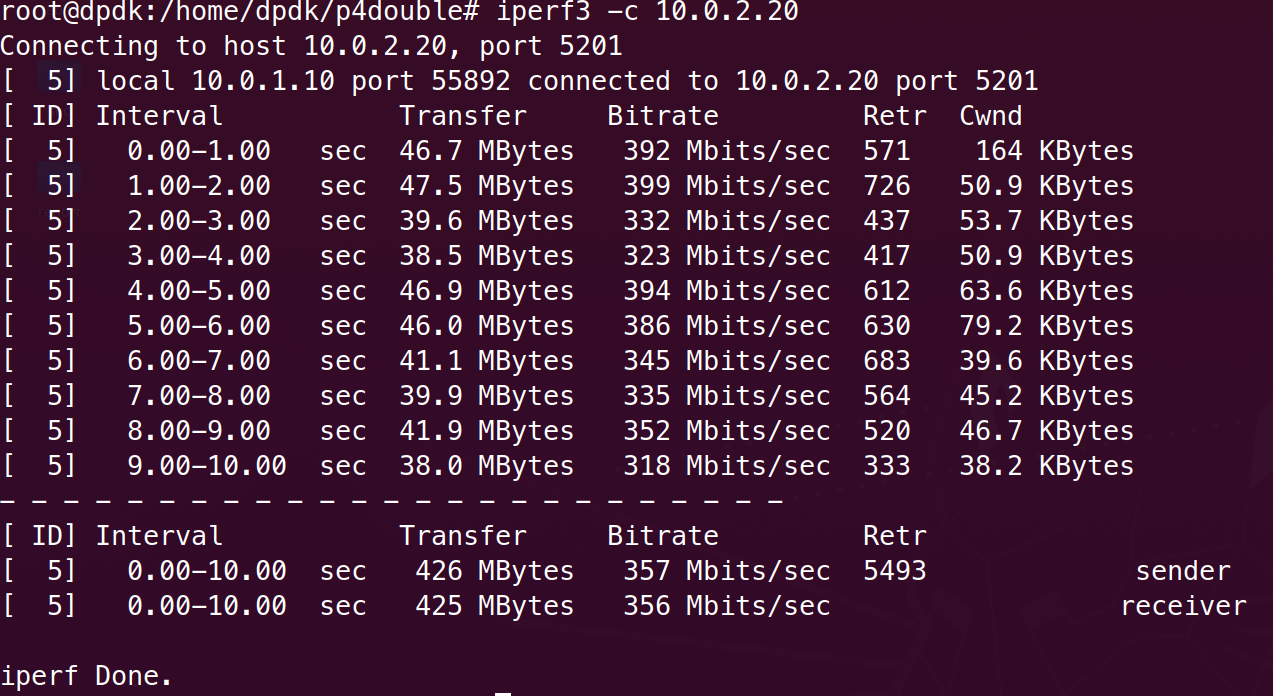
\includegraphics[width=7.5cm]{images/h1_p4double_patrick.png} }}%
    \qquad
    \subfloat[\centering H2]{{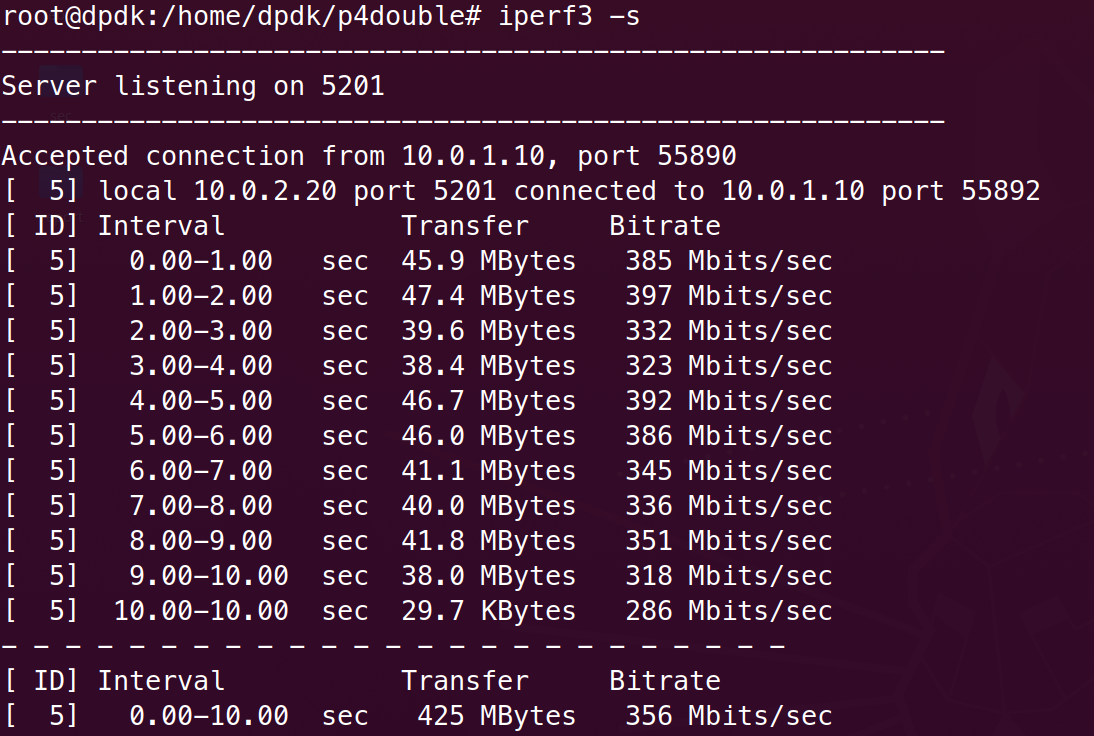
\includegraphics[width=7cm]{images/h2_p4double_patrick.png} }}%
    \caption{P4 double switch}%
    \label{fig:h1_p4double_patrick}%
\end{figure}
\FloatBarrier

\subsection*{Considerazioni}
\addcontentsline{toc}{subsection}{Considerazioni}
I test in \textbf{{Figura \ref{fig:h1_p4basic_patrick}}}
 mostrano le prestazioni di un semplice forwarding. Le prestazioni sono poco sotto il Gigabit in TX (\textbf{{Figura \ref{fig:h1_p4basic_patrick}.a}}) e in RX (\textbf{{Figura \ref{fig:h1_p4basic_patrick}.b}}) perché in condizioni ideali su un host reale non virtualizzato, BMv2 ha un throughput medio di 1047 Mbit/s \cite{noauthor_behavioral_2022}. È quindi ordinario aver un basso bitrate a causa del target su cui si esegue il programma P4, che è infatti solo a scopo di test. 
\leavevmode\newline
\\
Nei test in \textbf{{Figura \ref{fig:h1_p4double_patrick}}} si sottolinea come le prestazioni calano significativamente aggiungendo in cascata un ulteriore switch. In \textbf{{Figura \ref{fig:h1_p4double_patrick}.a}} sono presenti i test di trasmissione, in \textbf{{Figura \ref{fig:h1_p4double_patrick}.b}} sono presenti i test in ricezione.
\leavevmode\newline
\\
Il target BMv2 può avere scarse prestazioni per diversi motivi, alcuni dei quali possono essere i seguenti
\begin{itemize}
    \item Performance dell'hardware sottostante
    \item La complessità del programma P4 caricato: all'aumento della complessità del programma segue l'aumento della latenza
    \item Il compilatore utilizzato per generare il JSON
    \item Utilizzo in macchina virtuale
\end{itemize}
\subsection*{Problematiche}
\addcontentsline{toc}{subsection}{Problematiche}
Durante il setup dell'ambiente, dopo aver testato il ping tra i namespace H1 e H2, si può procedere testando le prestazioni con il software IPerf3 \cite{noauthor_iperf_nodate}. Durante questa fase è stato difficile capire perché i dispositivi non riuscissero a stabilire una connessione sfruttando questo tool. Uno dei motivi possibili per spiegare questo evento è che durante il tragitto attraverso gli switch, il parser e il deparser di BMv2 andassero a modificare il checksum degli header IPv4. Per risolvere il problema è possibile disabilitare il \textbf{TCP checksum offloading}, che serve per controllare la validità del checksum degli header.
È possibile disabilitare tale funzionalità su entrambi gli host attraverso il seguente comando, utilizzando ethtool \cite{noauthor_ethtool8_nodate}. In questo modo è possibile sfruttare IPerf3 con il protocollo TCP \cite{noauthor_cant_nodate}.
\begin{minted}{bash}
ethtool -K ethX rx off tx off
\end{minted}
\pagebreak
\section*{Punti aperti e sviluppi futuri}
\addcontentsline{toc}{section}{Punti aperti e sviluppi futuri}

\addcontentsline{toc}{subsection}{P4Pi}
\subsection*{P4Pi}
In futuro sarebbe interessante studiare tecnologie e altri target P4. Un progetto di nome P4Pi \cite{noauthor_getting_2022} porta la compatibilità di P4 sui Raspberry Pi, dei Single Board Computer economici. Così facendo sarebbe possibile agganciare in modo ``Plug and Play" a delle reti questi dispositivi così da poterli utilizzare come switch o router.\\

\addcontentsline{toc}{subsection}{OVS-P4}
\subsection*{OVS-P4}
Un altro progetto che estende le funzionalità di P4 è OVS-P4 \cite{osinski_p4-ovs_2022}. Lo scopo di questa estensione di P4 è quella di incrementare le prestazioni degli switch P4 tramite OpenVSwtich sfruttando tecnologie come uBPF \cite{noauthor_ubpf} e DPDK.
Questo è possibile perché la modifica a livello di Data Plane appare trasparente a OVS che continua a comportarsi come switch ma con prestazioni di inoltro maggiori.
OVS, come nella sua versione standard, può implementare DPDK, beneficiando dei vantaggi di forwarding che questo framework offre. Sfruttando DPDK non è più necessario separare user-space e Kernel, ma è possibile implementare accanto allo switch virtuale i metodi di Kernel Bypassing. In questo modo si completano in user-space Data Plane e Control Plane, così da avere un bypass completo del Kernel. \\
OVS sfrutta così DPDK ma mantiene anche la versatilità offerta dai programmi P4 applicati ai virtual switch di cui dispone.
In \textbf{{Figura \ref{fig:ovs_dpdk}}}
 si notano le differenze tra l'utilizzo di OVS con e senza DPDK.
\vspace{2cm}
\FloatBarrier
\begin{figure}[h]
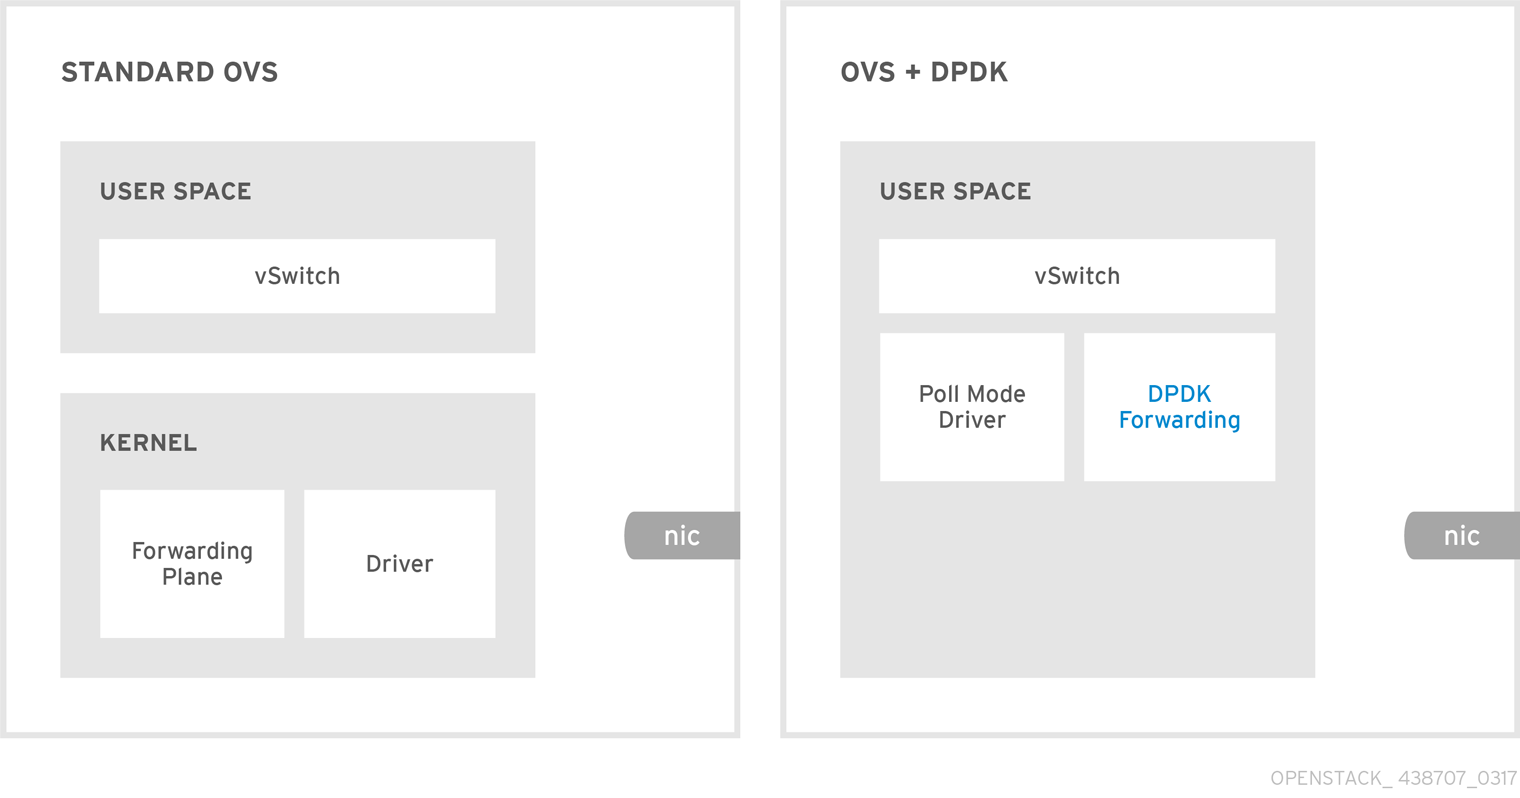
\includegraphics[scale=0.27]{images/ovs_dpdk.png}
\centering
\caption{\textit{OVS and OVS with DPDK}}
\label{fig:ovs_dpdk}
\end{figure}
\FloatBarrier

\addcontentsline{toc}{subsection}{T4P4S}
\subsection*{T4P4S}
T4P4S (Translator for P4 Switches) è un progetto che ha lo scopo di generare codice P4 ad alte prestazioni \cite{noauthor_p4elte_nodate}. Il compilatore P4 genera un file JSON, T4P4S esegue il parsing e genera codice C che viene poi collegato alle API di DPDK. Questo compilatore sfruttando le API generiche di C riesce a garantire prestazioni elevate, arrivando a superare le prestazioni di OVS+DPDK nei benchmark di forwarding, quindi a puro livello di Data Plane.
In \textbf{{Figura \ref{fig:t4p4s}}} si nota la pipeline di compilazione di un programma P4 in codice C per lo specifico target.
\FloatBarrier
\vspace{1cm}
\begin{figure}[h]
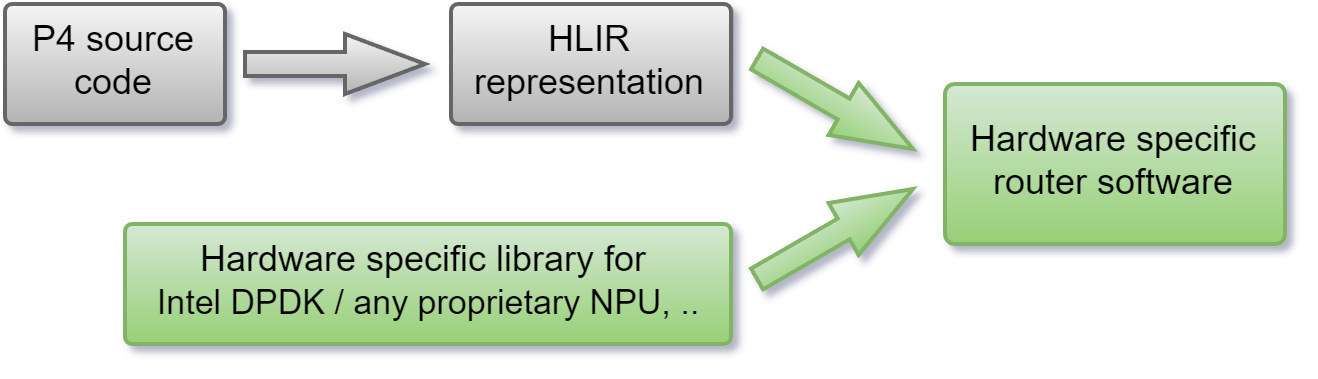
\includegraphics[scale=0.40]{images/t4p4s.png}
\centering
\caption{\textit{T4P4S Compiler}}
\label{fig:t4p4s}
\end{figure}
\FloatBarrier
\leavevmode\newline
La compilazione segue un modello a pipeline. Si inizia da una rappresentazione intermedia (Intermediate Rapresentation) che sarà poi compilata in codice C grazie alle API del Network Hardware Abstraction Layer. È il Core Compiler che si occuperà di generare il codice per lo specifico target, sfruttando le NetHAL API calls. Il Core di T4P4S implementa infatti il ``Packet Parsing" e le ``Actions" di P4 e traduce il tutto in funzioni C.

\pagebreak

\section*{Ambiente di Test}
\addcontentsline{toc}{section}{Ambiente di Test}

\subsection*{Computer Host}
\addcontentsline{toc}{subsection}{Computer Host}
La macchina host su cui sono stati eseguiti i test e su cui sono state lanciate le macchine virtuali dispone dei seguenti requisiti hardware

\begin{itemize}
    \item CPU: I5 6600K 4 Core 4 Thread 64 Bit
    \item RAM: 16 GB 2900MHz
    \item S.O: Linux Ubuntu 20.04 LTS
    \item NIC: Intel Ethernet 1219-V full duplex 1GBit/s
\end{itemize}

\subsection*{Virtual Machine}
\addcontentsline{toc}{subsection}{Virtual Machine}
Le Virtual Machine sono copie di una singola macchina virtuale con le seguenti specifiche
\begin{itemize}
    \item CPU: 2 Cores
    \item RAM: 4GB
    \item S.O: Linux Ubuntu 20.04 LTS
    \item HDD: 50GB
\end{itemize}

\subsection*{Virtualizzazione}
\addcontentsline{toc}{subsection}{Virtualizzazione}
\begin{itemize}
    \item Software di Virtualizzazione: QEMU/KVM \cite{noauthor_qemu_nodate}
    \item Paravirtualized drivers: VirtIO
    \item Device Drivers: MacVTap
\end{itemize}



